\documentclass[10pt,twocolumn,letterpaper]{article}
\usepackage[review]{cvpr}
\usepackage{times}
\usepackage{amsmath,amssymb,booktabs,graphicx}
\usepackage{tikz}
\usetikzlibrary{positioning,arrows.meta}
\usepackage[pagebackref,breaklinks,colorlinks]{hyperref}
\def\paperID{0000}
\def\confName{CVPR}
\def\confYear{2027}
\title{AutoSimSOTA: Autonomous Research over Native Simulation Repositories}
\author{Anonymous authors}
\begin{document}
\maketitle
\begin{abstract}
Can autonomous research extend beyond prepared experiment templates to native
robotics simulation repositories? We study a repository-level workflow in which
a main agent connects resources and native evaluation, establishes a baseline,
and chooses between gathering diagnostic information, acquiring training
experience, and changing learning or deployment methods. Simulation is both an
experimental feedback source and, where supported, a source of lawful training
experience. Trusted execution preserves resource limits, evaluated artifact
identity and independent evaluation while the agent retains research decisions.
Failure-directed acquisition and selection form a domain-specific branch, not a
mandatory stage. We specify separate system-level comparisons and controlled
data studies, including complete costs, failures and operator interventions.
\textbf{Development draft: matched system comparisons, transfer experiments and
data-intervention controls remain pending. Observed development gains are not
held-out gains, evidence of a data-method effect, or public SOTA results.}
\end{abstract}

\section{Introduction}
Autonomous simulation research requires more than changing a model in an already
connected training script. Native repositories differ in resource layouts,
control interfaces, learning workflows, expert availability and evaluation
semantics. The research problem is to reconstruct executable interventions and
decide what experiment is worth its full cost, without replacing the task judge.
Useful next steps may obtain information, obtain training experience, or modify
the learner or its lawful deployment. No single route is universally appropriate.

Robot imitation learning depends on the distribution of demonstrations available
to the learner. A policy can achieve low training loss and still fail at states
underrepresented in its demonstrations. Simulation offers an opportunity to
generate additional supervision, but a runnable simulator alone is not an expert:
a usable acquisition pipeline also needs task initialization, valid expert actions,
success and termination semantics, serialization, and a compatible training loader.
Acquiring more trajectories therefore involves both a learning decision and a
repository integration problem.

Scalable generation systems such as MimicGen provide powerful mechanisms for
expanding demonstrations~\cite{mimicgen}. DataMIL demonstrates that selection
should be evaluated through downstream policy performance rather than assumed
useful from human notions of similarity~\cite{datamil}. RESample directly addresses
missing recovery supervision through coverage-guided augmentation~\cite{resample}.
These works make a weak novelty claim---``failure data are useful''---insufficient.
Our data-specific question is whether a repository-level workflow can turn
development failures into executable, resource-accounted interventions that
outperform matched acquisition controls. The broader system question is whether
an agent can construct and revise effective research routes across native
workflows with less manual integration and competitive end-to-end outcomes.

The workflow builds on the research-agent decomposition of AutoSOTA~\cite{autosota}, rather than
claiming a new agent architecture. Repository acquisition replaces paper-to-code
discovery. A specialized Data role investigates expert availability, acquisition
conditions, quality checks, conversion, provenance, and training consumption. The
main Scheduler remains responsible for decisions and execution; independent
supervision checks scientific validity. Human-readable run reports expose what
was actually attempted, what remains blocked, and what the evidence supports.

The intended contribution is an experimentally validated account of autonomous
research-route construction, adaptation and optimization in native simulation
repositories. Candidate mechanisms include source-grounded capability discovery,
evidence-conditioned intervention choice, short recoverable research loops, and
failure-directed data acquisition when useful. Their value requires comparisons
against capable generic agents and existing robotics autoresearch workflows;
module count or passing software tests cannot establish novelty or effectiveness.

\section{Related Work}
\paragraph{Autonomous experimentation.}
AutoSOTA supplies a research-agent decomposition~\cite{autosota}.
Autoresearch-robotics already supports iterative algorithm and architecture
rewrites, online RL experience collection, visual feedback and experiment memory
over prepared task templates~\cite{autoresearchrobotics}. We do not claim these
abilities are absent or novel by themselves. Matched-template optimization and
native-repository integration are separate experiments; any extended baseline
must receive comparable tools, visual capabilities and total resources, with
adaptation costs disclosed. Transfer beyond those templates remains to be tested.

\paragraph{Demonstration generation.}
MimicGen scales robot-learning data through generation from human demonstrations
across environments and tasks~\cite{mimicgen}. We do not introduce a replacement
motion planner or general expert. We investigate whether a research agent can
identify and connect a repository's existing generation mechanism, then choose
useful conditions within its supported training domain. A repository without a
valid automated expert is outside the autonomous acquisition track unless another
legitimate supervision mechanism is explicitly available.

\paragraph{Performance-aware selection.}
DataMIL uses datamodel-based reasoning and a task-specific surrogate to select
data for imitation learning~\cite{datamil}. Our present implementation does not
include its datamodel algorithm. It is a relevant comparator when its requirements
and cost fit the selected policy and task. We must establish whether failure-directed
acquisition adds value beyond quality filtering and performance-aware selection
of already available data.

\paragraph{Recovery supervision.}
RESample uses a conservative coverage function, exploratory sampling, and recovery
actions to supplement missing corrective supervision~\cite{resample}. Thus,
failure-guided recovery collection itself is not an unclaimed direction. Our
workflow must specify which native acquisition decisions are automated, what
evidence selects them, and whether automation generalizes to previously unseen
tasks or repositories. Unsupported actions are not relabeled as expert supervision.

\section{System and Data-Acquisition Branch}
\subsection{Repository-level research loop}
The main agent maintains a bounded working plan and selects relevant skills and
instructions on demand. It inspects current capabilities and prerequisites,
chooses a testable intervention, executes through the trusted native runner, and
uses measured feedback to retain, reject or revise the route. Specialists answer
concrete questions rather than enforce a fixed delegation sequence. Decisions
and artifact identities persist across restarts; observed facts, hypotheses and
unresolved conditions remain distinct. Optional reports or recordings must not
erase a committed measurement. These are implementation mechanisms, not evidence
that the complete system outperforms alternatives.

\begin{figure}[t]
\centering
\resizebox{\linewidth}{!}{%
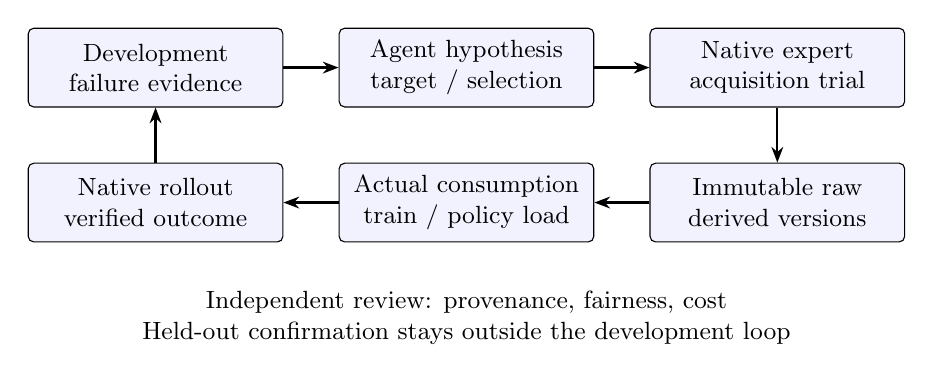
\begin{tikzpicture}[node distance=7mm and 7mm,
 box/.style={draw,rounded corners=2pt,align=center,font=\small,
             minimum height=10mm,text width=30mm,fill=blue!5},
 arrow/.style={-{Stealth[length=2mm]},thick}]
\node[box] (fail) {Development\\failure evidence};
\node[box,right=of fail] (plan) {Agent hypothesis\\target / selection};
\node[box,right=of plan] (collect) {Native expert\\acquisition trial};
\node[box,below=of collect] (data) {Immutable raw\\derived versions};
\node[box,left=of data] (train) {Actual consumption\\train / policy load};
\node[box,left=of train] (eval) {Native rollout\\verified outcome};
\draw[arrow] (fail)--(plan);
\draw[arrow] (plan)--(collect);
\draw[arrow] (collect)--(data);
\draw[arrow] (data)--(train);
\draw[arrow] (train)--(eval);
\draw[arrow] (eval)--(fail);
\node[align=center,font=\small,below=5mm of train] {Independent review: provenance, fairness, cost\\
Held-out confirmation stays outside the development loop};
\end{tikzpicture}}
\caption{The optional data-acquisition branch. Each edge needs native evidence;
an agent plan is not a successful acquisition or a verified performance gain.}
\label{fig:workflow}
\end{figure}
\subsection{Problem and capability boundary}
An input consists of an isolated source checkout, explicitly connected resources,
a native development evaluation protocol, and a total resource envelope. The
following notation concerns the data branch only; fixed-data, online RL and
deployment-only routes need not provide expert demonstrations. Let
$D_0$ denote available training demonstrations and $\pi_0$ the reproducible
baseline. Development rollouts provide evidence $E_t$. The agent proposes an
intervention $h_t=(g_t,q_t,m_t)$, where $g_t$ describes supported acquisition
conditions, $q_t$ specifies selection, and $m_t$ defines the training mixture.
These are research decisions, not a hard-coded benchmark recipe. Their source
connections must be established before execution.

More explicitly, an executable intervention specifies acquisition controls $g_t$,
task-directed selection $q_t$, an accepted-data target $n_t$, an actual training
mixture $m_t$, and completed learning work $u_t$. Controls must be connected to
native source and validated by a small acquisition trial. The task-directed
selector is distinct from a common validity floor $Q_0$ applied to every arm:
successful expert supervision, complete episode boundaries, aligned observations
and actions, legal training provenance, and source-family deduplication.
Accepted quantity is not attempted quantity; rejected acquisition and extra
samples collected for selection remain part of cost.

The current implementation uses source-grounded agent proposals rather than a
learned acquisition-value estimator. Failure observations, causal hypotheses,
and executable controls remain distinct. Low aggregate success alone does not
establish a coverage deficit, and a reset-only expert does not support claims of
mid-trajectory recovery acquisition.

The intended iteration is
\begin{equation}
 D_t^{+}=q_t(\operatorname{Collect}_{\mathrm{native}}(g_t)),
 \quad \pi_{t+1}=\operatorname{Train}(D_0,D_t^{+};m_t).
\end{equation}
The equation specifies an experiment, not a guarantee of a usable collector.
A small native acquisition trial must establish expert validity, complete-episode
output, serialization, and conversion before scaling. If these prerequisites
cannot be met within resources, the run reports that boundary. It does not claim
acquisition from a planned command or reinterpret failed learner actions as
successful expert trajectories.

\subsection{Agent decisions versus execution constraints}
The Scheduler maintains a persistent research plan and consults Data, Resource,
Init, Fix, and other roles as needed. Agents first see a short skill directory and
explicitly choose relevant procedures with reasons. Recommendations do not silently
replace agent choices. Data analyzes the connection between observed failure,
native expert capabilities, target conditions, quantity, quality, and loader
consumption. Resource reasons about local duration, storage, and cost; the Scheduler
can submit long jobs, inspect progress, revise local limits, or cancel stalled
jobs. The executor enforces only authorized total ceilings and experiment contracts.

This separation matters for portability: changing repositories should change
source-derived commands and proposals, not require a new hidden benchmark branch.
However, an unconstrained shell or self-modifying evaluator would invalidate
results. Skills and agents cannot override held-out separation, metric semantics,
unknown usage reservations, or immutable experiment evidence.

\subsection{Data identity and actual consumption}
Raw outputs are immutable research resources; filtering and conversion create
derived versions with parent identities and transformation provenance. A recorded
acquisition observation must have a verified native collection ancestor. Merely
processing an existing official dataset does not qualify as new acquisition.
The version registry connects each experimental arm to its acquired and training
versions, while the measurement records actual training consumption.

The chain to be verified is
\begin{center}
\small Native producer $\rightarrow$ raw data $\rightarrow$ derived view\\
$\rightarrow$ consumed training input $\rightarrow$ loaded policy\\
$\rightarrow$ native rollout $\rightarrow$ measured outcome.
\end{center}
Registering an intention or observing a checkpoint file is insufficient. Recorded
observations require verified policy consumption, rollout evidence, metric lineage,
and data consumption. One measurement cannot represent both targeted and random
arms, or multiple seeds. Evidence is checked again during export; changed data or
inconsistent native receipts exclude a row instead of producing a stale table.

\subsection{Campaigns and independent review}
A campaign records a development measurement, a falsifiable hypothesis,
acquisition and selection plans, required arms, accepted-episode budget, declared
training seeds, recipe, and cost-accounting intent. Its registration is not an
experiment result. A campaign observation joins a new scored measurement to its
native-produced data lineage. Scientific fairness is reviewed separately from
whether an individual score is genuine. Missing or insufficient review remains
uncertain; a real metric does not establish matched training exposure or fair cost.

\subsection{Evaluation separation and failure recovery}
Independent evaluation conditions are reserved before optimization, using
source-supported native inputs. A training RNG seed alone does not establish
disjoint initial conditions. Once search or measurement begins, the reservation
cannot be retroactively replaced. Held-out outcomes are not used to propose
acquisition targets or filter training data.

Execution failures are sealed with stable evidence identifiers. Fix receives the
actual command, outcome, and evidence rather than a shortened display message.
Valid replacements require a source/evidence connection and re-verification of
the failed operation. Framework development interventions are recorded separately;
trajectories that required such interventions cannot be described as uninterrupted,
frozen-system autonomous trials.

\section{Experimental Protocol}
\subsection{System comparisons}
Compare fixed native recipes, a capable generic research workflow, matched
autoresearch-robotics variants, and the complete system under equal end-to-end
resource envelopes. Report final native performance, completion rates, time to
the first verified score, best-score versus cost curves, failures and operator
interventions. Use at least three independent agent-research repeats in the
minimum main comparison; training seeds and evaluation episodes are different
levels of variation. Common templates and native-repository adaptation are
reported separately, with genuinely unseen repositories registered prospectively.
These experiments are planned, not completed system-level results.

\subsection{Feasibility before scale}
The system gate is baseline--intervention--native evaluation--retain/revert--next
experiment, using the route selected by the main agent. The data-branch gate is
a real native collection--conversion--training--evaluation cycle
on a repository with an automated expert. The pilot uses source isolation and
explicit read-only resource links, rather than copying every resource or assuming
that copying code preserves its runtime. It must produce genuinely new usable
episodes and show that the intended version reaches training. A runnable environment
or an old baseline score does not pass this gate.

After the pilot, freeze the harness, skill corpus, model configuration, resource
bindings, and protocol. Select additional tasks and an unseen repository according
to verified expert capabilities and available resources. Record exclusions before
viewing held-out results. Development repairs are allowed during feasibility but
must not silently enter formal trials.

\subsection{Controls and two resource tracks}
Table~\ref{tab:controls} defines the minimum controls. All arms share the native
policy family, initialization policy, official-data access, permitted training
domain, metric semantics, and common quality floor. The targeted arms may differ
in acquisition conditions, not in privileged test access or expert quality.

\begin{table}[t]
\centering\small
\begin{tabular}{@{}p{.29\linewidth}p{.63\linewidth}@{}}
\toprule
Arm & Purpose \\
\midrule
Official recipe & Reproducible fixed-data reference.\\
Continuation & No-new-data, equal-total-compute control.\\
Random expansion & New data without failure targeting.\\
Rule-targeted expansion & Fixed failure-frequency or coverage rule, common quality floor.\\
Agent-targeted expansion & Agent-selected native conditions, common quality floor only.\\
Targeted + selection$^{\dagger}$ & Additional Qt-increment track on the same target acquisition route/pool.\\
\bottomrule
\end{tabular}
\caption{Planned controls, not completed or frozen experiments.
$^{\dagger}$Task-directed selection is a separate incremental study.}
\label{tab:controls}
\end{table}

In the \emph{equal-data} track, targeted and random arms receive the same number
of accepted complete episodes. Report attempts, rejection rates, duplicates,
conversion losses, actual training exposure, and acquisition cost. Equal accepted
counts do not imply equal compute. In the \emph{equal-compute} track, charge failed
acquisition, conversion, training, evaluation, and research overhead against
matched envelopes; fixed-data continuation receives the corresponding opportunity.
GPU device-lease time, wall time, and model cost remain distinct quantities.

The provisional matrix contains four candidate native tasks, five controls and
three policy-training seeds (60 cells); it is not a completed experiment or a
frozen task selection. We first admit two verified tasks and compare the fixed-data
reference, fixed-data continuation, random acquisition, fixed rule targeting, and
agent targeting across three training seeds (30 cells with independently trained
baselines). All acquisition arms share $Q_0$; the rule baseline is required in this
first-stage design because beating random alone does not demonstrate a benefit
from LLM reasoning. Matched additional learning work and an equal-total-compute
envelope are distinct protocols, not interchangeable labels.
A separate six-method draft adds task-directed selection on the same target
acquisition route/pool (72 candidate cells, or 36 after admitting two tasks).
It tests the Qt increment without duplicating agent-targeted acquisition under
another name. Both drafts retain unresolved native protocol fields and empty
bindings; neither freezes a study nor authorizes compute. An acquisition-only
result cannot establish a selection benefit, and the title and claims must be
narrowed if only acquisition is validated.

\subsection{Replication and statistics}
Use at least three independently trained seeds for the small confirmed task set,
with matched initialization procedures. Training-seed replication with a fixed
acquired dataset is different from independent replications of the complete agent
acquisition loop. Report the former as policy variation, and evaluate the latter
separately where affordable. Pooling many evaluation episodes is not a substitute
for independent training seeds or independent agent trials.

Episode-level paired comparisons require recorded matching initial-state identities;
shared episode indexes or RNG labels are insufficient. Otherwise use unpaired
comparisons and state that limitation. Report effect sizes and uncertainty, not
just the best run. A descriptive mean across declared seed IDs does not establish
that those seeds were actually used; independent source and receipt audit is required.

\subsection{Reporting and attribution}
Each run maintains a Chinese human-readable report with status, actual scored
comparisons, data progress, plots, and available native demos. Missing measurements
are displayed as pending, not zero success. Paper exports are read-only, content-
addressed snapshots. They distinguish whole-run costs from per-arm costs and
development evidence from frozen formal evidence. Manual fixes, restarts,
research choices, and unknown usage reservations are disclosed.

\section{Development Evidence and Pending Comparative Experiments}
The current implementation provides campaign provenance, consumption checks,
confirmation reservation, independent review interfaces, and development exports.
Software contract tests verify these mechanisms but are not embodied performance
results. The development runs have not yet supplied the matched data-intervention
comparisons needed for the main results table. Missing experiments remain
unreported rather than being filled with zero or historical debugging scores.

\subsection{Development case: autonomous deployment tuning}
On the RoboSyn \texttt{click\_bell} task, the locally trained ACT baseline achieved
24 successes in 100 development episodes. The agent proposed executing the full
16-action predicted chunk instead of 8 actions before querying the model again.
The resulting candidate reused the identical frozen policy weights, performed no
new training, and achieved 32 successes in a subsequent 100-episode development
evaluation. Both records declare the same task, random setting, episode count,
and evaluation seed (0); the intervention changes policy execution behavior,
not the task success predicate or metric definition.

\begin{table}[t]
\centering\small
\begin{tabular}{@{}lr@{}}
\toprule
Development measurement & Successes / episodes \\
\midrule
Locally trained ACT baseline & 24 / 100 \\
Agent-selected full-chunk execution & 32 / 100 \\
Released-weight local reference$^{\dagger}$ & 55 / 100 \\
\bottomrule
\end{tabular}
\caption{Development case, not the formal data-intervention main table.
$^{\dagger}$The released-weight reference is a separate local measurement;
its protocol comparability and official reproduction status require further audit.}
\label{tab:development-case}
\end{table}

The observed increase is 8 percentage points over the local baseline. It is a
single development comparison, selected during search, with no independent
training-seed or agent-run replication. Matching seed labels do not establish
paired initial states, and we make no statistical-significance claim. Independent
confirmation did not execute: source-state identity checks rejected the operation
before rollout. Thus no held-out success rate is available.

The proposal and candidate evaluation were system decisions, but the enclosing
development run required operator framework repairs and restarts; it is not an
uninterrupted frozen-system autonomous trial. A timed-out collection attempt
left 69 episode parquet files, but those outputs were not shown to be consumed
by the scored candidate. The increase is therefore not evidence for the proposed
failure-driven acquisition and selection mechanism. Nor does it establish SOTA:
the separate released-weight measurement is higher, and independent confirmation
and comparable strong baselines remain necessary. The case demonstrates an
observed local development gain from agent-selected deployment tuning while
also exposing source-identity and failure-reporting limitations of the harness.

\subsection{Prospective pilot: recovery, local gain and deployment control}
In a separate development track, a locally trained ACT policy completed 40,000
updates and obtained 4 successes in 20 native episodes with an execution horizon
of 16. After operator repairs to the artifact handoff, the agent recovered another
already-completed 40,000-update producer using its complete native bundle; a new
190.3-second evaluation also obtained 4/20, without repeating its earlier
3077.5-second training. This recovery is system feasibility evidence, not a
data-method gain or an independent replication.
The other two previously unscored producers were also recovered without
retraining, obtaining 4/20 and 1/20 in 192.3 and 213.5 seconds, respectively.
All three are same-requested-seed instrumentation-development candidates with
distinct policy identities, not independent training-seed replicates or data
intervention arms; the lower result is retained rather than excluded.

The agent then reused the baseline's identical frozen weights and tested an
execution horizon of 8. This deployment-only control obtained 2/20 in 211.4
seconds, compared with the baseline's 4/20 in 192.3 seconds, and the system
reverted the candidate. This is a negative single-seed development observation;
matching seed labels do not establish paired initial states, and no significance
claim is made. Neither comparison used newly acquired training data.

In a subsequent diagnostic candidate, the agent selected an update-boundary
instrumentation patch and a local work budget of 2,000 updates at batch size 8.
It recovered the complete bundle from that same producer, scored 6/20 in a
179.9-second native evaluation, and explicitly retained the 30\% development
result against the 20\% baseline. The original failed handoff remains recorded.
This compound intervention changed both instrumentation and learning work;
without isolated controls or verified data consumption, the observed ten-point
gain cannot establish a data-method effect or a shorter-training advantage.
Training logs also exposed malformed interleaved witness records and missing
reader/stage metadata, which remain data-adapter limitations, not evidence of
verified batch consumption. No held-out or significance claim is made.

The same track completed a native expert collection with 20 saved demonstrations
from 20 reported attempts: 1480 time steps and 60 videos across three cameras,
in 1025.1 seconds of process time. Operator read-only checks verified format,
numerical and video-timestamp consistency. These checks are not autonomous expert
quality certification; collection success is not learned-policy success, and the
new pool has not yet supplied a verified training-consumption and performance
comparison. This pilot therefore supports data-supply feasibility, not the
effectiveness of failure-driven targeting, MimicGen, or DAgger.

The eventual analysis must answer: does targeting improve success at equal data
quantity; does it retain an advantage at equal total cost; which failures are
recoverable by the native expert; and do decisions transfer to held-out tasks or
repositories without operator intervention? Ablations should remove failure
targeting and task-directed selection separately, holding the remaining procedure
constant. Additional policies or more repositories are useful only if the core
comparison is already reproducible.

\subsection{Recovered candidate in the required-data track}
In a separate prospective RoboSyn track with 50 development episodes, the main
agent resumed an already completed training producer whose initial handoff had
failed at the policy-artifact boundary. It selected the native handoff correction
and evaluated the original producer without retraining. The recovered candidate
obtained 9/50 (18\%), compared with this track's baseline of 6/50 (12\%); the new
evaluation exited normally in 445.6 seconds. Independent receipt checks matched
the loaded policy identity, all 50 completed rollouts and the reported metric.
The original failed handoff remains recorded.
This is a single-seed development observation after operator budget and service
maintenance, with data consumption still unverified. It supports recovery
feasibility, not an acquisition effect, statistical significance or a held-out
gain, and is not pooled with the earlier 20- or 100-episode tracks.

\paragraph{Released-policy calibration.}
The main agent separately evaluated released ACT revision
\texttt{677e65f} on 50 development episodes, obtaining 24/50 (48\%)
without retraining, in 316.3 seconds. Receipt verification matched the loaded
policy, completed rollouts and native metric. The reference registry accepted
this reading under its previously reviewed detection band of 0.14 around the
documented 37\%; that band is not a statistical equivalence test. The reference
and local-baseline logs share 50 episode IDs, but identical physical initial
states have not been independently established. This calibration is neither an
agent-discovered improvement nor a new-data result, and does not replace the
local baseline or enter the formal comparison table. It establishes that the
local evaluation chain can distinguish a stronger released policy, while the
causes of the short-trained local policies' lower performance remain hypotheses.

\paragraph{A negative diagnostic candidate.}
On October 16 the main agent also recovered a 1,000-update batch-instrumentation
candidate without retraining, obtaining 4/50 (8\%) with verified policy loading,
rollouts and metric lineage. The incumbent remained 18\%. An earlier detached
probe of the same policy obtained 6/50 (12\%); we do not replace the lower formal
record, pool these attempts, or treat them as independent research repetitions.
Physical initial-state pairing and registered-data consumption remain unverified.
This observation supports handoff recovery, not a data-acquisition benefit or
performance improvement.

\paragraph{Longer-training development intervention.}
On October 17 Main independently selected 80,000 optimizer updates on the existing
data. Training completed in 6,153.1 seconds with a source-audited terminal counter.
After a file-versus-bundle handoff refusal, Fix diagnosed the boundary and Main
selected the complete producer bundle without retraining. The unchanged
50-episode protocol yielded 12/50 (24\%) in 413.3 seconds, with verified loading,
rollouts and metric lineage. This exceeds the local 12\% baseline and previous
18\% development observation, but uses more learning work and remains below the
48\% released-policy reference. All 38 failures were labelled insufficient
contact/press. No data-method effect, paired significance, held-out gain or
public SOTA is established. The measurement was initially saved but unadopted
when maintenance paused the run. Main subsequently adopted the same result
after rechecking sealed receipts and archived bytes, updating the incumbent
from 18\% to 24\% without retraining or another evaluation.

\subsection{Fixed-policy action-execution ablation}
On October 19, in the prospective RoboSyn \texttt{click\_bell} track, Main
established a local development baseline of 56/100. It then hypothesized that
replanning more frequently would remedy insufficient contact/press failures.
The candidate changed only the deployment configuration, executing four rather
than fifty actions per ACT query. It reused the exact baseline policy bundle,
without additional training. Both conditions used the unchanged evaluator,
\texttt{random} setting, seed zero, and the same ordered 100 episode seeds.
Initial-state hashes were not recorded, so we do not claim physical-state pairing.

\begin{table}[t]
\centering
\small
\setlength{\tabcolsep}{4pt}
\begin{tabular}{lrrr}
\toprule
Actions/query & Successes & Queries/ep. & Eval. seconds \\
\midrule
50 (baseline) & 56/100 & 4.42 & 674.2 \\
4 (Agent candidate) & 0/100 & 91.00 & 1293.6 \\
\bottomrule
\end{tabular}
\caption{A fixed-policy development ablation. More frequent replanning did not
improve this policy; this is not a data-intervention or SOTA result.}
\label{tab:fixed-policy-execution}
\end{table}

The candidate completed all episodes with normal process exit. All 100 failures
were classified by the native diagnostic as insufficient contact/press; the
baseline had 44 such failures. Mean action steps increased from 196.8 to 361.0.
Total policy queries increased 20.59-fold, whereas evaluation wall time increased
1.92-fold. These are different cost measures, not a 20-fold end-to-end slowdown.
The hypothesis was unsupported under these development conditions, and the
56\% incumbent was retained. The result illustrates why deployment intuition
requires native outcome and cost feedback; it does not establish a general
causal explanation or benefit of our data-acquisition method.

The first score lookup failed because a legacy archive basename differed from
the frozen result locator. After operator maintenance of the CPU recovery
interface, Main and Fix corrected the request and source citations; an independent
review linked the same completed native evaluation without replay. Read-only
receipt verification passed for both measurements, including identical frozen
policy identity and parent lineage. Operator repairs and restarts must therefore
be included in system cost: this is not an unassisted end-to-end comparison.

\subsection{External native-port baseline pilots}
We conducted preliminary native-repository integration pilots using ENPIRE's
public research contract and interfaces~\cite{enpire}, and
autoresearch-robotics' public research instructions~\cite{autoresearchrobotics}.
The pinned source revisions are \texttt{99ee90ac} and \texttt{ff30cc48},
respectively. These are adapted instruction-driven ports, not reproductions of
the original systems' complete experimental configurations. The ENPIRE RoboTwin
port actually invokes its \texttt{TrialRunner} and \texttt{ArtifactStore}; the
RoboSyn ports follow its contract around native batch evaluation rather than
using its complete runtime. Neither port uses AutoSimSOTA's research agents,
skills or candidate-approval pipeline.

\paragraph{Conditions.}
All arms use DeepSeek Flash in non-thinking mode, with at most 8192 output tokens
per request, one RTX 5090, isolated editable code and read-only existing resources.
Each arm has a \$5 model cap and a 75-minute cumulative research window, including
integration. Development uses 20 episodes with seed 2026; the separate confirmation
seed is 2027 with 50 episodes. RoboSyn uses the released ACT policy on
\texttt{click\_bell/random}; RoboTwin uses an existing locally trained ACT
checkpoint on \texttt{beat\_block\_hammer/demo\_clean}, not a reproduced official
baseline. After an initial rendering failure, both RoboTwin ports fix the native
default/raster shader switch before their scored runs. This condition is not
claimed equivalent to the benchmark's default ray-traced rendering.
Operators supplied environment, transport and recording repairs, all logged.
An initial text-only RoboSyn diagnostic is separate from four subsequently
image-enabled arms; enabling image input does not imply a blocked arm actually
obtained visual feedback.

\begin{table*}[t]
\centering\small
\begin{tabular}{@{}lllll@{}}
\toprule
Adapted research workflow & Task repository / feedback & Baseline & Candidates & Retained-policy confirmation \\
\midrule
ENPIRE contract & RoboSyn / text diagnostic & 11/20 & 10/20; 6/20 & 21/50 (unchanged baseline) \\
ENPIRE native interfaces & RoboTwin / image-enabled & 0/20 & 0/20; 0/20 & Not run \\
autoresearch-robotics & RoboTwin / image-enabled & 0/20 & 0/20; 0/20; 0/20 & Not run \\
autoresearch-robotics & RoboSyn / image-enabled & Unavailable & Not evaluated on random & Not run on random \\
ENPIRE contract & RoboSyn / image-enabled & Unavailable & Not evaluated on random & Not run on random \\
\bottomrule
\end{tabular}
\caption{External native-port pilot observations, reported as successes/episodes.
Unavailable scores denote failure before a valid task evaluation, not zero
success. Each row is a single development research run, not a replicated system
comparison. Candidate and baseline measurements are not pooled with earlier
AutoSimSOTA development cases or with off-protocol diagnostics.}
\label{tab:external-native-pilots}
\end{table*}

\paragraph{Measured interventions.}
In the text-only RoboSyn diagnostic, the agent shortened the ACT execution
horizon from 50 to 25 and 10 actions, obtaining 10/20 and 6/20 versus 11/20.
Both candidates were rejected; the unchanged baseline then obtained 21/50 on
seed 2027. Native per-episode records agree with all four aggregate scores.
A later temporal-ensembling probe obtained 7/20 but occurred after confirmation
had begun; it is retained as exploratory evidence, not a frozen candidate result.

On RoboTwin, the ENPIRE port tried the best-validation checkpoint and disabling
temporal aggregation; both yielded 0/20, as did its baseline. All 60 episode
records terminate at the native 400-step limit, with no wrapper-error outcomes.
The autoresearch-robotics port tried enabling temporal aggregation, retraining
ACT on 50 existing demonstrations, and combining retraining with aggregation.
All four evaluations yielded 0/20 in the native evaluator, with completed
episode counters and successful checkpoint-load logs. Retraining completed
400 epochs in 356.3 seconds; it did not acquire new data. Its report names
\texttt{policy\_best.ckpt}, but actual evaluation logs show
\texttt{policy\_last.ckpt}. We report the executed policy identity and do not
attribute the best-validation loss to the deployed checkpoint. No improved
candidate was selected or confirmed on RoboTwin.

\paragraph{Blocked protocols and diagnostic controls.}
Both image-enabled RoboSyn arms failed before establishing the requested
\texttt{random} baseline. Logs show native material initialization assertions or
hangs in distractor-mesh loading. The autoresearch-robotics port additionally
produced minimal multi-mesh failure probes. A separate \texttt{clear} diagnostic
obtained 12/20 with the released policy, 3/20 after shortening its execution
horizon to 25, and 12/20 after setting \texttt{act\_step=5}; a seed-2027 baseline
diagnostic obtained 32/50. The ENPIRE image-enabled arm completed only a
\texttt{clear} smoke test (1/1). These measurements use a different scene
configuration and do not replace the missing \texttt{random} scores. Because the
earlier text arm did run \texttt{random}, the blocked arms do not establish that
RoboSyn is inherently unsupported: the relevant environment difference remains
unresolved. The agent's declaration of a terminal boundary is not itself proof
that the failure cannot be repaired without changing the task.

\paragraph{Interpretation and audit boundary.}
These pilots demonstrate some executable integration and candidate rejection,
but no improved native score, new-data benefit, or public SOTA. RoboTwin's two
ports start with different aggregation defaults, and accepted expert-valid
initial-state seed vectors differ across some evaluations. Thus the shared
top-level seed does not establish paired physical starts or a matched system
ranking. Small samples, one research run per condition, operator setup changes
and the chosen model configuration preclude general capability conclusions.
Independent exports retain 17 native measurements with source paths and hashes,
checkpoint-load discrepancies, unavailable protocol outcomes and costs. The
five arms have \$0.4993 of provider-priced model usage, plus a separate vision
preflight; an additional \$0.1426 unsettled reserve remains in the text arm and
is not counted as a settled charge or silently released. These figures are not
complete hardware or operator costs. Source-code identity checks on the two
original repositories are unchanged. The launcher also missed a report written
under \texttt{benchmark/} and omitted some native output formats from its status
index; the paper uses actual artifacts rather than those incomplete counters.

\section{Limitations and Submission Gate}
Automated acquisition is not supported by every simulation repository. Missing
assets, incompatible hardware, absent expert supervision, or non-reproducible
baselines may prevent experiments. Source citations do not prove successful
runtime integration. Likewise, agent-generated plans do not prove that acquired
data cover the identified failures or improve a learned policy.

The current pilot is a development run with documented framework intervention,
not formal evidence of complete autonomy. A submission needs matched system
comparisons, full-cost controls, independent research repeats, held-out evaluation
and evidence of the claimed native-workflow adaptation. Data-method claims
additionally need matched acquisition controls and an incremental mechanism
beyond existing selection and recovery methods.
If those gates fail, the scope or submission timeline should change. The paper
must not substitute a broad framework narrative for missing experimental evidence.

{\small
\bibliographystyle{ieeenat_fullname}
\bibliography{references}
}
\end{document}
